
\section{Les ensembles de nombres.}

\subsection{Ensembles fondamentaux de nombres}

$\mathbb{N}$ est l'ensemble des nombres entiers  : $ 3 \in \N $ et $-3 \notin \N$

$ \Z $ est l'ensemble des nombres entiers relatifs (vient de "zahlen" = les nombres en allemand) : \\ $ 3 \in \Z, -4 \in \Z $ mais $ -4 \notin \N $ \\

On a : $ \N \subset \Z $ \\


$ \Q $ est l'ensemble des nombres rationnels : $ 3 \in \Q, -4 \in \Q, \dfrac{3}{4} \in \Q $ mais $ \dfrac{3}{4} \notin \N $ et $ \dfrac{3}{4} \notin \Z $

On a : $ \N \subset \Z \subset Q $ \\

\underline{Remarque :} $ \D $ est l'ensemble des nombres décimaux : $ \dfrac{3}{4} = 0,75 $ donc $ \dfrac{3}{4} \in \D $ mais  $ \dfrac{4}{3} = 1,333... $ \\ d'où $ \dfrac{4}{3} \notin \D $ \\ 

On a : $ \N \subset \Z \subset \D \subset Q $ \\

$ \R $ est l'ensemble des nombres réels : $ 3 \in \R, -4 \in \R, \dfrac{3}{4} \in \R, \dfrac{4}{3} \in \R, \sqrt{2} \in \R $ \\ mais $ \sqrt{2} \notin \N, \sqrt{2} \notin \Z, \sqrt{2} \notin \Q $. \\

On a : $ \N \subset \Z \subset \Q \subset \R $ \\

\underline{Remarque :} \\ $ \pi \in \R $ \\
$ \sqrt{2} $ est un nombre irrationnel  (c'est-à-dire qu'il est solution d'une équation algébrique à coefficients entiers) ; on peut avoir : $ x^{2} = 2 $ \\

$\pi $ est un nombre irrationnel transcendant. 

$ e $ est un nombre irrationnel transcendant. \\

$ \C $ est l'ensemble des nombres complexes (aussi appelés nombres imaginaires ou nombres impossibles)

$ \imath \in \C $ 

$ \imath^2 = -1 $

\newpage

\subsection{Intervalles}

\subsubsection{Définition}

Soient $ a \in \R $ et $ b \in \R $ avec $ a < b $ \\

$ \left[ a, b \right] $ est l'ensemble des nombres réels x tels que $ a\leqslant x\leqslant b $. C'est un intervalle fermé. \\

% [a, b]  intervalle fermé
\begin{tikzpicture}
     \tkzInit[xmin=-30,xmax=20,xstep=6]
     \tkzDrawX[label={},noticks,nograd]
     
     \tkzXHW[color=green]    % I=]-10,7[
     {
      -30/T//-10/T/[,        % On hachure  de -inf à -10
        7/T/]/20/T/          % et de 9 à +inf
     }
     \tkzText(-10,-.5){a}    % Etiquette gauche
     \tkzText(7,-.5){b}      % Etiquette droite
     \tkzText(0,0){\textcolor{red}{$\times$}}  % Etiquette croix sur R
     \tkzText(0,-.3){\textcolor{red}{$x$}}     % Etiquette x sous croix
\end{tikzpicture}

$ \left] a, b \right[ $ est l'ensemble des nombres réels x tels que $ a\ < x\ < b $. C'est un intervalle ouvert. \\

% ]a, b[  intervalle ouvert
\begin{tikzpicture}
     \tkzInit[xmin=-30,xmax=20,xstep=6]
     \tkzDrawX[label={},noticks,nograd]
     
     \tkzXHW[color=green]    % I=]-10,7[
     {
      -30/T//-10/T/],        % On hachure  de -inf à -10
        7/T/[/20/T/          % et de 9 à +inf
     }
     \tkzText(-10,-.5){a}    % Etiquette gauche
     \tkzText(7,-.5){b}      % Etiquette droite
     \tkzText(0,0){\textcolor{red}{$\times$}}  % Etiquette croix sur R
     \tkzText(0,-.3){\textcolor{red}{$x$}}     % Etiquette x sous croix
\end{tikzpicture}

$ \left[ a, b \right[ $ est l'ensemble des nombres réels x tels que $ a\ \leqslant x\ < b $. C'est un intervalle semi-ouvert à  droite. \\

% [a, b[  intervalle  semi ouvert à droite
\begin{tikzpicture}
     \tkzInit[xmin=-30,xmax=20,xstep=6]
     \tkzDrawX[label={},noticks,nograd]
     
     \tkzXHW[color=green]    % I=]-10,7[
     {
      -30/T//-10/T/[,        % On hachure  de -inf à -10
        7/T/[/20/T/          % et de 9 à +inf
     }
     \tkzText(-10,-.5){a}    % Etiquette gauche
     \tkzText(7,-.5){b}      % Etiquette droite
     \tkzText(0,0){\textcolor{red}{$\times$}}  % Etiquette croix sur R
     \tkzText(0,-.3){\textcolor{red}{$x$}}     % Etiquette x sous croix
\end{tikzpicture}

$ \left] a, b \right] $ est l'ensemble des nombres réels x tels que $ a\ < x\ \leqslant b $. C'est un intervalle semi-ouvert à  gauche. \\

% semi ouvert à gauche
\begin{tikzpicture}
     \tkzInit[xmin=-30,xmax=20,xstep=6]
     \tkzDrawX[label={},noticks,nograd]
     
     \tkzXHW[color=green]    % I=]-10,7[
     {
      -30/T//-10/T/],        % On hachure  de -inf à -10
        7/T/]/20/T/          % et de 9 à +inf
     }
     \tkzText(-10,-.5){a}    % Etiquette gauche
     \tkzText(7,-.5){b}      % Etiquette droite
     \tkzText(0,0){\textcolor{red}{$\times$}}  % Etiquette croix sur R
     \tkzText(0,-.3){\textcolor{red}{$x$}}     % Etiquette x sous croix
\end{tikzpicture}


\subsubsection{Extension de la notion d'intervalle :}

$ \left]-\infty , a \right] $ est l'ensemble des nombres réels x tels que $ x \leqslant a. $

% x <= a (Inférieur ou égal) 
\begin{tikzpicture}
     \tkzInit[xmin=-30,xmax=20,xstep=6]
     \tkzDrawX[label={},noticks,nograd]
     
     \tkzXHW[color=green]    % I=]-10,7[
     {
        7/T/]/20/T/          % On hachure  de -inf à 7
     }
     \tkzText(7,-.5){a}      % Etiquette gauche
     \tkzText(0,0){\textcolor{red}{$\times$}}  % cf ci-dessus
     \tkzText(0,-.3){\textcolor{red}{$x$}}
      
\end{tikzpicture}

$ \left]-\infty , a \right[ $ est l'ensemble des nombres réels x tels que $ x < a. $ \\

% x < a (Strictement inférieur) 
\begin{tikzpicture}
     \tkzInit[xmin=-30,xmax=20,xstep=6]
     \tkzDrawX[label={},noticks,nograd]
     
     \tkzXHW[color=green]    % I=]-10,7[
     {
        7/T/[/20/T/          % On hachure  de -inf à 7
     }
     \tkzText(7,-.5){a}      % Etiquette gauche
     \tkzText(0,0){\textcolor{red}{$\times$}}  % cf ci-dessus
     \tkzText(0,-.3){\textcolor{red}{$x$}}
      
\end{tikzpicture}


$ \left[ a, +\infty \right[ $ est l'ensemble des nombres réels x tels que $ x \geqslant a. $ \\

% x >= a
\begin{tikzpicture}
     \tkzInit[xmin=-30,xmax=20,xstep=6]
     \tkzDrawX[label={},noticks,nograd]
     
     \tkzXHW[color=green]    % I=]-10,7[
     {
       -30/T//-10/T/[       % On hachure  de -inf à -10
     }
     \tkzText(-10,-.5){a}    % Etiquette gauche
     \tkzText(0,0){\textcolor{red}{$\times$}}  % Etiquette croix sur R
     \tkzText(0,-.3){\textcolor{red}{$x$}}     % Etiquette x sous croix
\end{tikzpicture}

$ \left] a, +\infty \right[ $ est l'ensemble des nombres réels x tels que $ x > a. $ \\

% x > a
\begin{tikzpicture}
     \tkzInit[xmin=-30,xmax=20,xstep=6]
     \tkzDrawX[label={},noticks,nograd]
     
     \tkzXHW[color=green]    % I=]-10,7[
     {
       -30/T//-10/T/]       % On hachure  de -inf à -10
     }
     \tkzText(-10,-.5){a}    % Etiquette gauche
     \tkzText(0,0){\textcolor{red}{$\times$}}  % Etiquette croix sur R
     \tkzText(0,-.3){\textcolor{red}{$x$}}     % Etiquette x sous croix
\end{tikzpicture}








$ \left] -\infty, +\infty \right[ = \R $ \\

% ] -inf, +inf [
\begin{tikzpicture}
     \tkzInit[xmin=-30,xmax=20,xstep=6]
     \tkzDrawX[label={},noticks,nograd]
     \tkzText(0,0){\textcolor{red}{$\times$}}  % Etiquette croix sur R
     \tkzText(0,-.3){\textcolor{red}{$x$}}     % Etiquette x sous croix
     
\end{tikzpicture}

\newpage

\subsubsection{Intersection d'intervalles}

\textbf{Exemple \no 1}

$ I = \left[-3, 5 \right[ $ et $ J = \left] 2, 8 \right] $ \\

% ex 1 Intersection I=[-3, 5[ n J=]2, 8]
\begin{tikzpicture}
     \tkzInit[xmin=-5,xmax=10,xstep=1.8] % Le pas fixe la longueur
     \tkzDrawX[label={},noticks,nograd]
     
     \tkzXH[color=green]    % I=]-3, 5[
     {
      -5/T//-3/T/[,
        5/T/[/10/T/
     }
     \tkzText(-3,-.5){-3}
     \tkzText(5,-.5){5}
      \tkzXHW[color=red]   % J=]2, 8]
     {
        -5/T//2/T/],   % On retire de -inf à -21 
         8/T/]/10/T/        % et de 9 à +inf
     }
     \tkzText(2,-.5){2}
     \tkzText(8,-.5){8}
\end{tikzpicture}

$ I \cap J $ est l'ensemble des nombres réels qui appartiennent à  $ I $ \textbf{et}   $ J $  \\

$ I \cap J = \left] 2,5 \right[ $ \\

\textbf{Exemple \no 2}

$ I = \left]-10, 7 \right[ $ et $ J = \left[ -21, 9 \right[ $ \\

% ex2
\begin{tikzpicture}
     \tkzInit[xmin=-30,xmax=20,xstep=6]
     \tkzDrawX[label={},noticks,nograd]
     
     \tkzXH[color=green]    % I=]-10,7[
     {
      -30/T//-10/T/],
        7/T/[/20/T/
     }
     \tkzText(7,-.5){7}
     \tkzText(9,-.5){9}
      \tkzXHW[color=red]   % J=[-21,9[
     {
      -30/T//-21/T/[,   % On retire de -inf à -21 
        9/T/[/20/T/        % et de 9 à +inf
     }
     \tkzText(-21,-.5){-21}
     \tkzText(-10,-.5){-10}
\end{tikzpicture}

$ I \cap J = \left] -10,7 \right[ $ \\

\underline{Remarque :} $ I \cap J = I $ car $ I \subset J $ \\

\textbf{Exemple \no 3}

$ I = \left[-7, 3 \right] $ et $ J = \left] 5, 11 \right[ $ \\

% ex3
\begin{tikzpicture}
     \tkzInit[xmin=-10,xmax=15,xstep=3]
     \tkzDrawX[label={},noticks,nograd]
     \tkzXHW[color=red]
     {
         -10/T//-7/T/[, % On retire de -inf à -7 
           3/T/]/15/T/  % et de 3 à +inf
     }
     \tkzText(-7,-.5){-7}
     \tkzText(3,-.5){3}
     \tkzXH[color=green]
     {
      -10/T//5/T/],
       11/T/[/15/T/
     }
     \tkzText(5,-.5){5}
     \tkzText(11,-.5){11}
        
\end{tikzpicture}

$ I \cap J = \varnothing $ (l'ensemble vide)

\subsubsection{Réunion d'intervalles}

\textbf{Exemple \no 1} 

$ I = \left[1,5 \right] $ et $ J= \left[4,9 \right[ $ \\

$ I \cup J $ est l'ensemble des nombres réels $ x $ tels que $ x \in I $ \textbf{ou} $ x \in J $ \\

% ex 4 I=[1,5] J=[4,9[
\begin{tikzpicture}
     \tkzInit[xmin=-0,xmax=10,xstep=1.2]  % Definit la portion dans R
     \tkzDrawX[label={},noticks,nograd]   % Trace l'axe 
% I=[1,5]                                 
     \tkzText(1,0){\bf [}      % Place le crochet gauche en 1
     \tkzText(5,0){\bf ]}      % Place le crochet droit en 5
     \tkzDefPoint(1,.05){I1}   % Nomme I1 le point gauche 
     \tkzDefPoint(5,.05){I2}   % Nomme I2 le point droit 
     \tkzDrawSegments[color=red](I1,I2) % Trace l'intervalle en rouge
     \tkzText(1,-.5){1}        % Etiquette gauche
     \tkzText(5,-.5){5}        % Etiquette droite
% J=[4,9[     
      \tkzText(4,0){\bf [}     % Place le crochet gauche en 4 
     \tkzText(9,0){\bf [}      % Place le crochet droit en 9
     \tkzDefPoint(4,-.05){J1}  % Nomme J1 le point gauche 
     \tkzDefPoint(9,-.05){J2}  % Nomme J2 le point droit
     \tkzDrawSegments[color=green](J1,J2) % Trace l'intervalle en vert
     \tkzText(4,-.5){4}        % Etiquette gauche
     \tkzText(9,-.5){9}        % Etiquette droite
        
\end{tikzpicture}

$ I \cup J = \left[1,9\right[ $ \\

\textbf{Exemple \no 2}

$ I = \left]-1,3 \right[ $ et $ J= \left]6,10 \right] $ \\

% ex 5 I=]-1,3[ J=]6,10]
\begin{tikzpicture}
     \tkzInit[xmin=-3,xmax=12,xstep=1.2]  % Definit la portion dans R
     \tkzDrawX[label={},noticks,nograd]   % Trace l'axe 
% I=]-1,3[                                 
     \tkzText(-1,0){\bf ]}      % Place le crochet gauche en -1
     \tkzText(3,0){\bf [}      % Place le crochet droit en 3
     \tkzDefPoint(-1,.05){I1}   % Nomme I1 le point gauche 
     \tkzDefPoint(3,.05){I2}   % Nomme I2 le point droit 
     \tkzDrawSegments[color=red](I1,I2) % Trace l'intervalle en rouge
     \tkzText(-1,-.5){-1}        % Etiquette gauche
     \tkzText(3,-.5){3}        % Etiquette droite
% J=]6,10]     
      \tkzText(6,0){\bf ]}     % Place le crochet gauche en 4 
     \tkzText(10,0){\bf ]}      % Place le crochet droit en 9
     \tkzDefPoint(6,-.05){J1}  % Nomme J1 le point gauche 
     \tkzDefPoint(10,-.05){J2}  % Nomme J2 le point droit
     \tkzDrawSegments[color=green](J1,J2) % Trace l'intervalle en vert
     \tkzText(6,-.5){6}        % Etiquette gauche
     \tkzText(10,-.5){10}        % Etiquette droite
        
\end{tikzpicture}

$ I \cup J = \left]-1,3\right[ \cup \left]6,10\right] $ \\

\underline{Remarque :} Dans ce cas, la réunion des deux intervalles n'est pas un intervalle, mais une réunion d'intervalles.
De plus, on a $ I \cap J = \varnothing $ \\

\newpage

\textbf{Exemple \no 3}

$ I = \left]3,5 \right[ $ et $ J= \left]-6,11 \right] $ \\

% ex 4 I]3,5[ J=]-6,11]
\begin{tikzpicture}
     \tkzInit[xmin=-7,xmax=12,xstep=1.5]  % Definit la portion dans R
     \tkzDrawX[label={},noticks,nograd]   % Trace l'axe 
% I=[1,5]                                 
     \tkzText(3,0){\bf ]}      % Place le crochet gauche en 1
     \tkzText(5,0){\bf [}      % Place le crochet droit en 5
     \tkzDefPoint(3,.05){I1}   % Nomme I1 le point gauche 
     \tkzDefPoint(5,.05){I2}   % Nomme I2 le point droit 
     \tkzDrawSegments[color=red](I1,I2) % Trace l'intervalle en rouge
     \tkzText(3,-.5){3}        % Etiquette gauche
     \tkzText(5,-.5){5}        % Etiquette droite
% J=[4,9[     
      \tkzText(-6,0){\bf ]}     % Place le crochet gauche en 4 
     \tkzText(11,0){\bf ]}      % Place le crochet droit en 9
     \tkzDefPoint(-6,-.05){J1}  % Nomme J1 le point gauche 
     \tkzDefPoint(11,-.05){J2}  % Nomme J2 le point droit
     \tkzDrawSegments[color=green](J1,J2) % Trace l'intervalle en vert
     \tkzText(-6,-.5){-6}        % Etiquette gauche
     \tkzText(11,-.5){11}        % Etiquette droite
        
\end{tikzpicture}

$ I \cup J = \left]-6,11\right] $ \\

\underline{Remarque :} $ I \cup J = J $ car $ I \subset J $


